
%Chapter 2

\renewcommand{\thechapter}{2}

\chapter{The LUX Detector}

\section{Introduction}

The LUX experiment is located 4850 ft underground at the Sanford Underground Research Facility. After running for 87 live days in 2013 LUX has recently set the most sensitive limit for a spin independent WIMP scattering cross section [ref] and is expected to achieve five times the sensitivity after a 300 day run in 2015. Nobel elements are ideal candidates for WIMP detection, they are easy to purify and are transparent to their own scintillation light. Xenon is especially favorable do to it's  large atomic mass (131.3 amu) and high liquid phase density ($\rm sim$2.9 kg/l) which provides both an excellent target for coherent WIMP scattering while simultaneously providing excellent shielding from external radioactivity. Xenon also has good radio purity with established techniques to remove and monitor troublesome radio isotopes of argon and krypton found in the atmosphere from which the xenon is distilled [refs]. 
WIMPs being electrically neutral would primarily interact with the xenon target nuclei producing nuclear recoils (NR) whereas typical backgrounds in the detector, gammas and betas, interact with the electrons producing electronic recoils (ER). In liquid xenon ER events can be further discriminated from NR events by about a factor of 1000 by taking the charge to light ratio of the interaction.



\section{The LUX TPC}

The LUX detector is a two phase xenon time projection chamber TPC,  [ref LUX inst]. . The detector contains two PMT arrays on the top and bottom with 61 PMTs each for a total of 122 PMTs, with quantum efficiencies ranging from 30-40\%. The active region consists of a 49 cm length between the cathode and gate with a 47 cm diameter of the dodecagonal geometry. The drift field between the cathode and gate is 180 V/cm resulting in an electron drift velocity of 1.51 mm/$\rm \mu s$. The liquid level terminates 5-6mm above the gate grid as the liquid xenon spills over into a weir reservoir. The anode grid is placed 1.0 cm above the gate grid and used to setup the electron extraction field of 6 kV/cm where electrons are removed from the liquid and accelerated causing electroluminescence in the gas phase.  LUX contains a gross 350 kg of xenon of which 250 kg are in the active region and 118 kg fiducial. A schematic of the detector in shown in ...

 \begin{figure}[h!]\centering
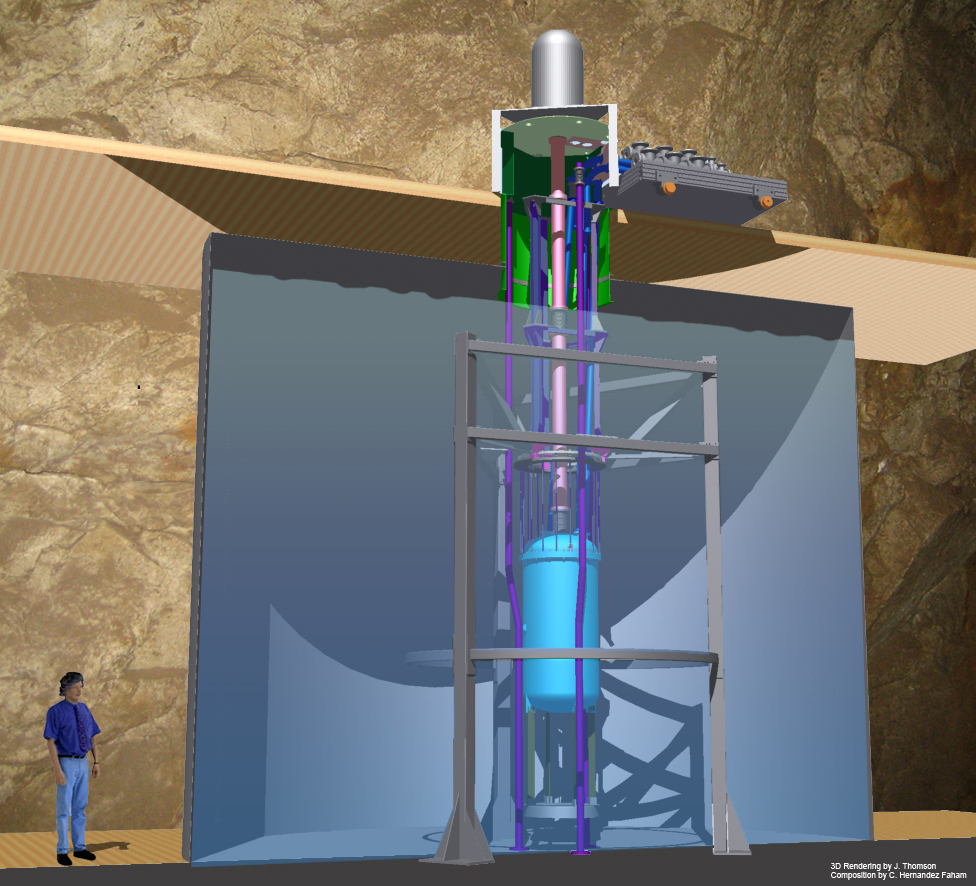
\includegraphics[scale=0.35]{Chapter_LUX_Det/Davis_3D_tank.jpg}
\caption{Schematic of the LUX detector and the surrounding water tank.}
\label{fig:LUX_Davis}
\end{figure}

 \begin{figure}[h!]\centering
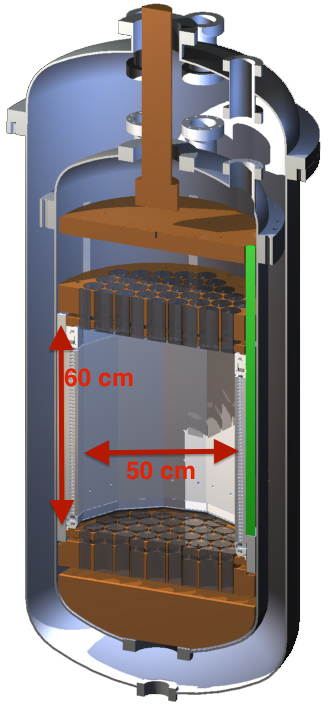
\includegraphics[scale=0.5]{Chapter_LUX_Det/LUX_half_rendering_white.jpg}
\caption{LUX Detector.}
\label{fig:LUX_TPC}
\end{figure}

%Add self shielding plot... 5 orders of magnitude reduction in the center.


\section{The Light and Charge Signals}

When energy is deposited in the active region of the xenon TPC it is converted to excitation, ionization and heat. For a given energy deposit, NR events lose a significant portion of energy to heat leaving less energy available for excitation and ionization than an ER event. Xenon excitons de-excite on the order of nano seconds producing 175nm VUV scintillation light, recombining ion electron pairs also emit scintillation light. The two channels for photon production overlap and sum to produce the primary scintillation signal (S1), arriving within 10s of ns as the photons are collected the  PMT arrays. Electrons which escape recombination with their ion pair feel the effect of the drift field and begin to drift upwards towards the gas phase phase (drift times of 0-324 $\rm \mu s$). Once extracted into the gas the electrons accelerate and electroluminece  producing a much larger secondary scintillation signal (S2), proportional the the number of electrons extracted. A schematic of an NR and ER event is shown in figure \ref{fig:TomS_ER}, figure \ref{fig:TomS_ER} and an illustration of an energy deposition in the LUX detector is show in figure \ref{fig:LUX_Event}. The timing separation between the S1 and S2 pulse is used to define the drift time and the hit pattern of the S2 signal on the top PMT array is used to define the XY position of the event. From the S1 and S2 signals the full x,y,z position and energy deposit of the event can be reconstructed.
%Show prompt fraction plot to describe event selection.



 \begin{figure}[h!]\centering
 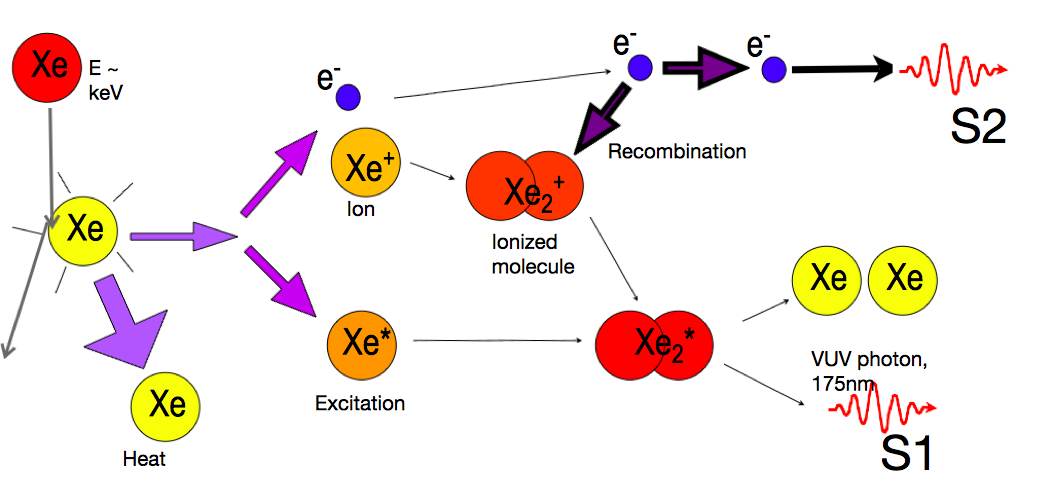
\includegraphics[width=150mm]{Chapter_LUX_Det/NR_T_Shutt.png}
\caption{Nuclear recoil (NR) event in xenon.}
\label{fig:TomS_ER}
\end{figure}

 \begin{figure}[h!]\centering
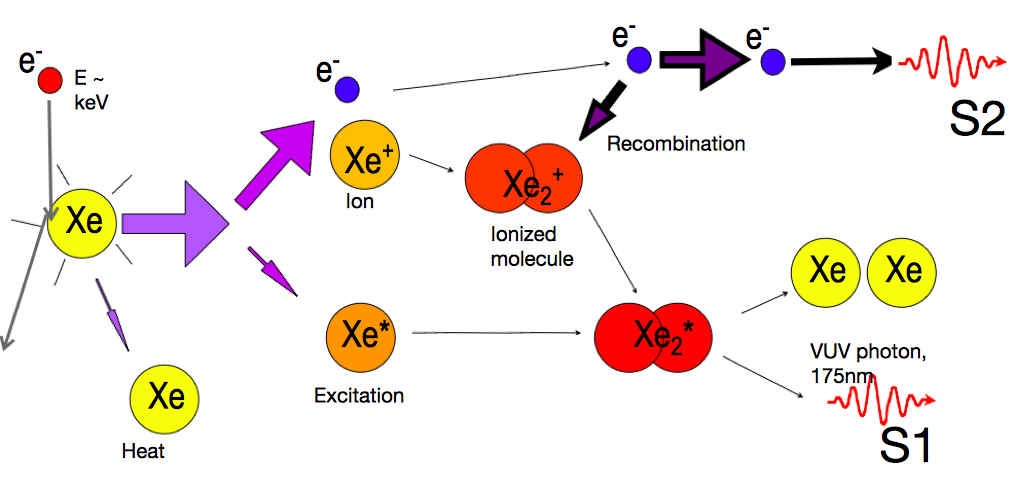
\includegraphics[width=150mm]{Chapter_LUX_Det/ER_T_Shutt.png}
\caption{Electronic recoil (ER) event in xenon}
\label{fig:TomS_NR}
\end{figure}

 \begin{figure}[h!]\centering
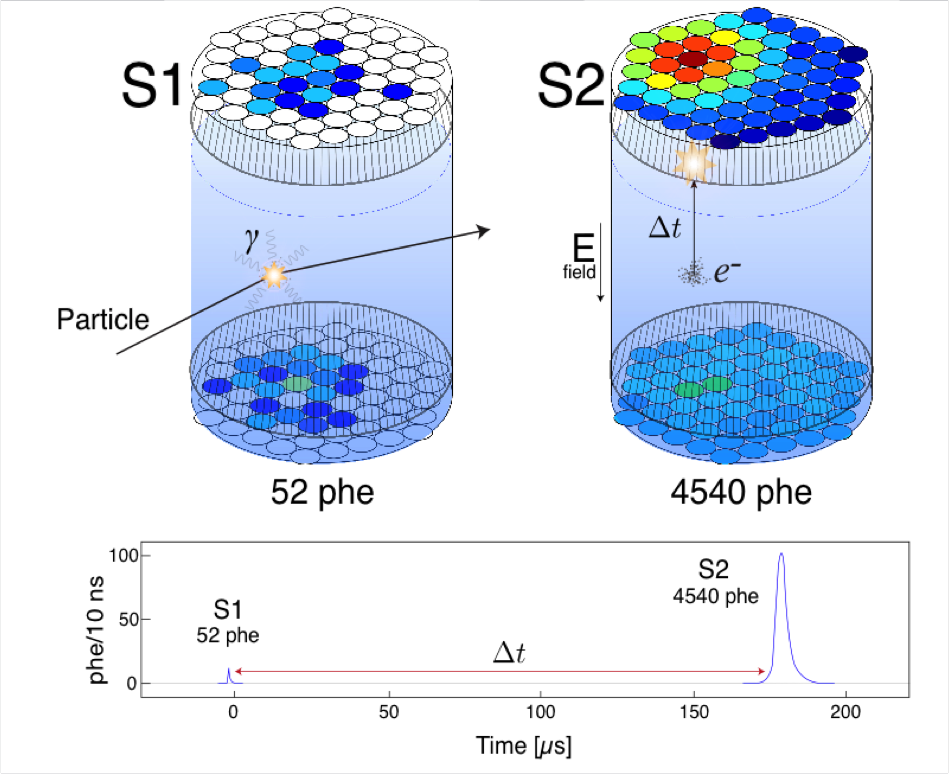
\includegraphics[width=150mm]{Chapter_LUX_Det/LUX_Event_Diagram.png}
\caption{Event diagram.}
\label{fig:LUX_Event}
\end{figure}

\section{Identifying S1, S2}
The primary and secondary signals have unique properties which can be used to identify their populations. The S1 signal is a fast spike summed along the PMT arrays, the signal decays in 10s of nano seconds as the primary scintillation and recombining election ion pairs emit photon VUV (175nm). The S2 signal arrives several $\rm \mu s$ later with the electron population spread out about the centroid of the interaction due to diffusion. The characteristic S2 signal is one with a slow rise and corresponding fall, resembling a bell curve. A 2 keV event as seen by all 122 PMT channels is showing in figure \ref{fig:LUX_Golden}, the s1 pulse is spiked as the photons arrive and the S2 pulse is much larger with a slower lifetime (the S2 pulse is larger since a single election creates hundred of photons as it is accelerated in the extraction region). 

%Show prompt fraction plot to describe event selection.

 \begin{figure}[h!]\centering
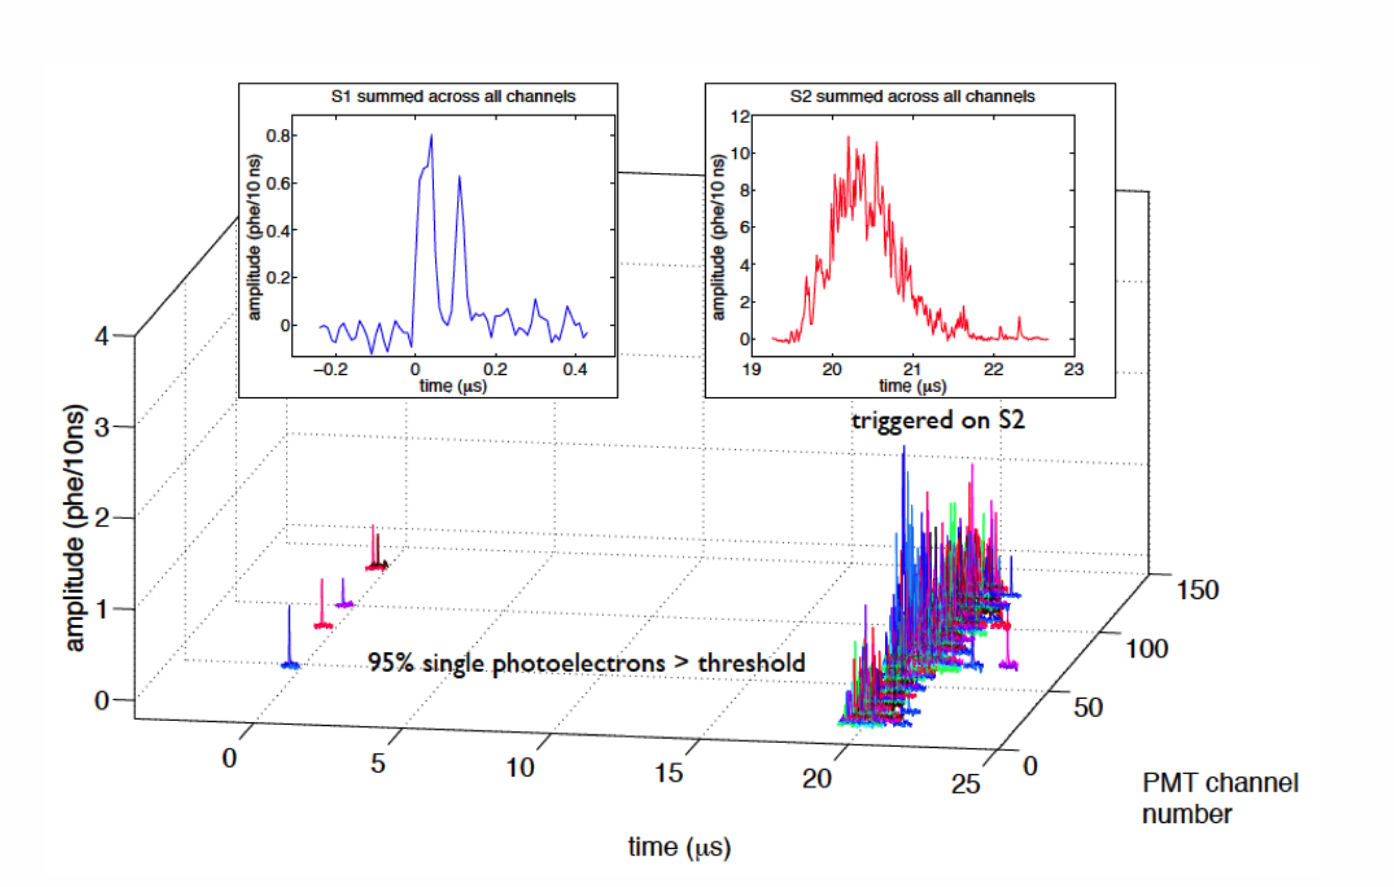
\includegraphics[width=150mm]{Chapter_LUX_Det/LUX_Golden_Event_2keV.png}
\caption{LUX 2keV ER event.}
\label{fig:LUX_Golden}
\end{figure}

To to the pulse characteristics of S1 and S2 we define a variable Prompt Fraction that traces the area covered in the fist 10\% of the pulse. For S1s this value will approach 1 and for S2s the value will be below 0.1, this provides for a powerful separation of the populations. The separation of population is shown in figure for the case of a $\rm ^{83m}Kr$ data set (41.5 keV gamma) and a tritium calibration data set (1-18.5 keV beta decay). The populations of single photons, single electrons, S1s and S2s are clearly visible and well speparted when plotting the prompt  fraction variable vs. pulse area (PE). Golden events for the WIMP search are single scatters which contain one S1 paired with a subsequent S2 pulse. Each single scatter golden event has a well defined x,y coordinate and z from the drift time. Golden events are corrected for detector geometry and electron attenuation, discussed in the next section.

 \begin{figure}[h!]\centering
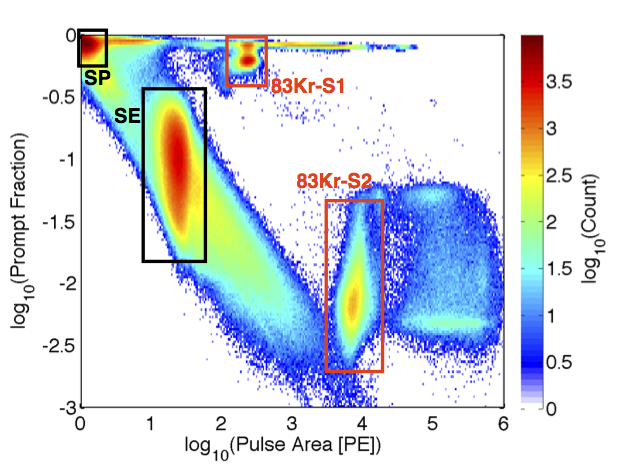
\includegraphics[width=120mm]{Chapter_LUX_Det/Kr_83_Density_text.png}
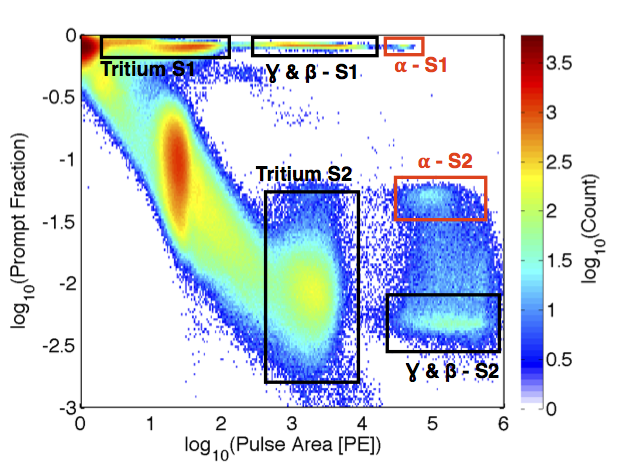
\includegraphics[width=120mm]{Chapter_LUX_Det/T_Density_text.png}
\caption{Density plot}
\label{fig:Prompt_Fraction}
\end{figure}


%Show S2/S1 plots from PRL and LUX result?
